%Instruções
% 1 - o pré ambulo esta arrumado para um formato padrão;
% 2 - Não mexer no arquivo main.

\chapter{Estatística Descritiva}

\section{Conceitos Gerais}

\inic A estatística é o ramo da ciência que tem por finalidade coletar, organizar, analisar e interpretar dados, os quais podem ser gerados a partir de indivíduos de diferentes categorias. Esses indivíduos podem representar bactérias, neurônios, células, ou quantidades de crimes.

Neste material, apresentamos diversas técnicas de análise de dados envolvendo os três principais ramos da Estatística: descritiva, probabilística e inferencial. Pretende-se abordar o conteúdo em nível de graduação, com enfoque em aplicações em diversas áreas do conhecimento, como Administração, Física, Gestão Ambiental, Matemática e Biologia, sem perder o rigor das definições e dos resultados estatísticos fundamentais.

Como referências principais, utilizamos \cite{morettin2017estatistica} e \cite{da1981curso}.

\begin{defin}[População]
População é o conjunto de indivíduos que apresentam pelo menos uma característica em comum.
\end{defin}

\noindent \exemplo
\begin{enumerate}
    \item[(i)] O conjunto de pessoas que torcem para o clube A. Um pesquisador pode estudar a proporção de homens e mulheres nessa população;
    
    \item[(ii)] O conjunto de pessoas com renda acima de R\$ 1.000,00. Um banco pode analisar essa população para definição de crédito;
    
    \item[(iii)] O conjunto de tipos de solos existentes em uma região. Um engenheiro pode analisar quais são adequados para construção civil;
    
    \item[(iv)] O conjunto de pessoas de uma cidade com conhecimento sobre reciclagem;
    
    \item[(v)] A população de carros de um determinado modelo, para análise de defeitos mecânicos.
\end{enumerate}

\inic Os exemplos acima ilustram aplicações da Estatística em diversas áreas do conhecimento. Destaca-se ainda a \textit{Mecânica Estatística}, área da Física na qual a Estatística é amplamente utilizada.

\begin{defin}[Amostra]
Uma amostra é um subconjunto da população.
\end{defin}

\noindent \exemplo
\begin{enumerate}
    \item[(i)] No conjunto de torcedores do clube A, pode-se selecionar uma amostra de indivíduos de diferentes faixas etárias;
    
    \item[(ii)] No estudo de solos, analisa-se apenas uma parte representativa do solo;
    
    \item[(iii)] Em pesquisas sociais, utiliza-se uma amostra da população para inferência estatística;
    
    \item[(iv)] Em engenharia automotiva, seleciona-se uma amostra de veículos para análise de falhas.
\end{enumerate}

\inic Em muitos casos, não é possível ou não é conveniente analisar toda a população. Assim, utilizam-se amostras para inferir propriedades da população.

\inic Nem toda amostra é adequada para generalizações. Para isso existe a área de \textit{amostragem}, que será discutida posteriormente.

\section{Classificação de Variáveis}

\inic Variáveis são características observadas nos elementos de uma população.

\inic Chamamos de \textit{variável quantitativa} aquela que expressa uma medida numérica do fenômeno estudado.

\noindent \exemplo
\begin{enumerate}
    \item[(i)] Número de pessoas que entram em uma loja, com valores em $\mathbb{N} = \{0,1,2,3,\ldots\}$;
    
    \item[(ii)] Tempo de vida de uma lâmpada, $t \in [0,+\infty)$;
    
    \item[(iii)] Massa de uma amostra de solo.
\end{enumerate}

\inic As variáveis quantitativas podem ser classificadas em discretas e contínuas.

\begin{defin}[Variável Discreta]
Uma variável é discreta quando assume valores finitos ou enumeráveis.
\end{defin}

\begin{defin}[Variável Contínua]
Uma variável é contínua quando pode assumir qualquer valor em um intervalo da reta real.
\end{defin}

\noindent \exemplo
\begin{enumerate}
    \item[(i)] Número de mulheres em um grupo de 10 pessoas (discreta);
    
    \item[(ii)] Número de pessoas que entram em uma loja ao longo do tempo (discreta);
    
    \item[(iii)] Tempo de vida de um pneu (contínua);
    
    \item[(iv)] Peso de um objeto (contínua).
\end{enumerate}

\begin{defin}[Variável Qualitativa]
Uma variável qualitativa descreve características do objeto estudado, não sendo expressa numericamente.
\end{defin}

As variáveis qualitativas podem ser classificadas em:
\begin{itemize}
    \item \textbf{Nominais}: não possuem ordem;
    \item \textbf{Ordinais}: possuem ordem natural.
\end{itemize}

\noindent \exemplo
\begin{enumerate}
    \item[(i)] Sexo de uma pessoa: masculino ou feminino;
    
    \item[(ii)] Tipo de solo: arenoso, argiloso, humoso, calcário;
    
    \item[(iii)] Resposta a uma pergunta: sim ou não.
\end{enumerate}

\inic O gráfico apropriado para variáveis qualitativas ordinais é o gráfico de colunas, como mostrado na Figura \ref{fig:colunas}.

\begin{figure}[H]
    \centering
    \caption{Exemplo de gráfico de colunas}
    \label{fig:colunas}
    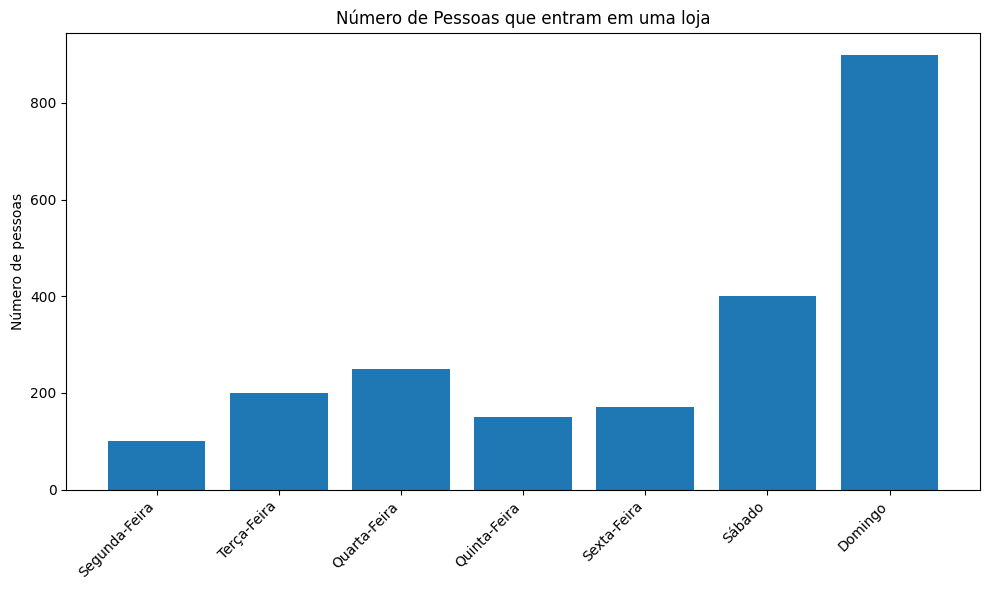
\includegraphics[scale=.6]{figuras/colunas}
\end{figure}

\inic Apresentaremos agora algumas formas de representação de amostras tento em vista a ordem de tabulação de dados. Diremos que os dados estarão organizados em ``Rol" se estes estiverem em ordem crescente ou decrescente. Em geral, um banco de dados $X =\{x_1,x_2, \cdots,x_n\}$ será representado como:

\begin{equation*}
    \begin{cases}
    x_{(1)}:\,\, \text{menor elemento da amostra};\\
    x_{(2)}:\,\,\text{2º menor elemento da amostra};\\
    \vdots\\
    x_{(n)}: \,\,\text{maior elemento da amostra.}\\
    \end{cases}
\end{equation*}
\inic Chamaremos de \textit{Amplitude} (h) o a diferença entre o maior e menor valor observado na amostra, isto é, $h = x_{(n)} - x_{(1)}$. Os gráfico apropriado para representamos dados em ordem crescente é o chamado \textit{gráfico de barras}, que é mostrado na Figura \ref{barras}

\begin{figure}[H]
    \label{barras}
	\centering
	\caption{Gráfico de Barras}
	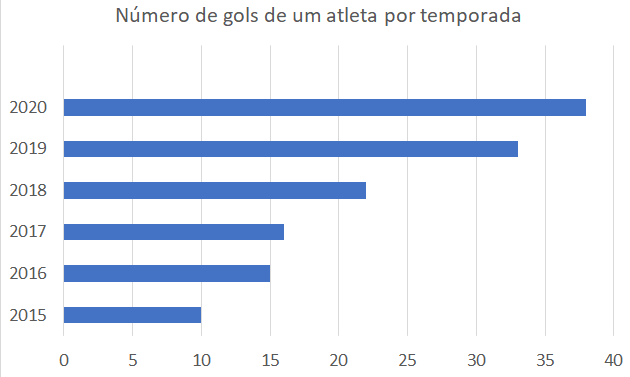
\includegraphics[scale=.6]{figuras/barras}
\end{figure}

\inic Note que a barras estão sempre na ordem crescente de quantidade de dados, o que caracteriza e diferença este gráfico.

\begin{defin}
Seja um banco de dados $X = \{x_1,x_2,x_3, \cdots, x_n\}$ chamamos de frequência absoluta ($f_i$) o número de vezes que o dado $x_i$ aparece na amostra.
\end{defin}
Vale salientar que cada $x_i$ pode ter diferentes significados, podendo até mesmo representar intervalos da reta (classes). O arranjo de valores com suas respectivas frequências é denominado \textit{Distribuição de Frequência}.

\noindent \exemplo
\begin{enumerate}
    \item[(i)] Em um hospital há cinco setores, a Tabela \ref{exemplo1} mostra a os leitos ocupados por setor:
\begin{table}[H]
    \caption{Generalização do crescimento simples}
    \label{exemplo1}
    \centering
    \begin{tabular}{cc}
    \hline
    Setor & $f_i$ \\
    \hline
    1 & 30 \\
    2 & 10 \\
    3 & 25 \\
    4 & 32 \\
    \hline
    \end{tabular}
\end{table}
\end{enumerate}
\inic Em geral tabelamos o par $(x_i, f_i)$ para melhor entendimento do leitor.
\section{Intervalos de Classe}
Agrupamos dados contínuos em intervalos de classes, que são definidos pelos símbolos ``$\vdash$" aberto a direita e fechado a esquerda e são distribuídos conforme a Tabela \ref{classes} 
	\begin{table}[H]
        \centering
        \caption{Intervalos de Classe}
        \label{classes}
		    \begin{tabular}{cc}
		    \hline
		    $\mathnormal{x_i}$ & $\mathnormal{f_i}$\\
		    \hline
		    35 $\vdash$ 45 & 5\\
		    45 $\vdash$ 55 & 12\\
		    55 $\vdash$ 65 & 18\\
	    	65 $\vdash$ 75 & 14\\
	    	75 $\vdash$ 85 & 6\\
	    	85 $\vdash \hspace{-0.2 cm }\dashv$ 95 & 3\\
		    \hline
		\end{tabular}
	\end{table}
	
Sendo $\vdash \hspace{-0.2 cm }\dashv$ intervalo fechado à direita e à esquerda. Os "$\mathnormal{f_i}$'s" \, representam a quantidade de valores que estão no intervalo indicado por $\mathnormal{x_i}$. a forma gráfica de representar intervalos de classe é dada pelos \textit{histogramas} que são gráficos conforme a Figura \ref{histo}
    
    \begin{figure}[H]
    \label{histo}
		\centering
		\caption{Histograma da Tabela \ref{classes}}
		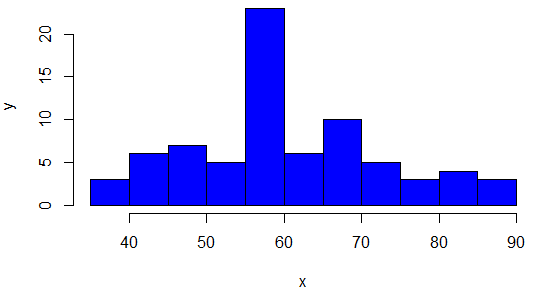
\includegraphics[scale=1]{figuras/histo}
	\end{figure}
	
\inic Posteriormente indicaremos o histograma como gráfico mais apropriado para entendermos como uma distribuição de probabilidade se comporta.

\section{Tabelas Estatísticas}
\inic Uma tabela estatística deve apresentar os seguintes elementos básicos:

\begin{enumerate}
	\item[(i)] Cabeçalho;
	\item[(ii)] Corpo, colunas e subcolunas da tabela;
	\item[(iii)] Rodapé, reservado para informações importantes da tabela.
\end{enumerate}
\inic Um bom cabeçalho deve responder os seguintes questionamentos:
\begin{enumerate}
	\item[(i)] O que está sendo representado?
	\item[(ii)] Onde ocorreu? 
	\item[(iii)] Quando ocorreu?
\end{enumerate}

\subsection{Série Temporal}
\inic Uma série de dados observado segundo a época de ocorrência:

\begin{table}[H]
    \centering
	\caption{Série temporal}
    \label{temporal}
	\begin{tabular}{cc}
		\hline
		Ano & Vendas\\
		\hline
		1970 & 2108 \\
		1971 & 1542 \\
		1972 & 3225 \\
    	1973 & 4788 \\
    	1974 & 1245 \\
		1975 & 3569 \\
		1976 & 4785 \\
		\hline
		\end{tabular}
		\\
	    Fonte: \cite{da1981curso}
	\end{table}
\subsection{Série Geográfica}
\inic É uma série estatística em que os dados são agrupados segundo modalidade de ocorrências 
\begin{table}[H]
    \centering
    \caption{Série Geográfica}
    \label{tab:my_label}
    \begin{tabular}{cc}
		\hline
		Regiões & Número\\
		\hline
		Norte & 7025 \\
		Nordeste & 107783 \\
		Sudeste & 218207 \\
		Sul & 15776 \\
		Centro-Oeste & 5243 \\
		\hline
	\end{tabular}
\end{table}
\subsection{Série Específica}
\inic É uma série estatística em que os dados são agrupados segundo modalidade de ocorrências, temos como exemplo a Tabela 
	\begin{center}
		\textbf{Matrículas no Ensino de Técnico Grau} \\
		\begin{tabular}{cc}
			\hline
			Áreas & Matrículas\\
			\hline
			Biologia & 32109 \\
			Agrárias & 107783 \\
			Letras & 2458 \\
			Artes & 3254 \\
			Histórias & 2451\\
			\hline
		\end{tabular}
		\\
		\textbf{Fonte}: \cite{da1981curso}
	\end{center}
\inic Note que a tabela representa a quantidade de indivíduos que obedecem a uma determinada categoria.
\section{Medidas de Tendência Central e de Posição}
\inic Buscamos estabelecer medidas para analisar os dados, buscamos valores que de fato consigam explicar a tendência e comportamento dos dados, apresentaremos nessa seção algumas medidas de tendência central e de posição que buscam explicar como os dados se comportam mediante a um determinado fenômeno, para explanar melhor definiremos o conceito de \textit{Média Arimética} de um banco de dados de tamanho $n$ dado por $X = \{x_1,x_2,x_3,\cdots,x_n\}$, de fato definimos média aritmética, denotada por $\overline{x}$ a expressão

\begin{equation}
\label{media}
    \overline{x} = \frac{\displaystyle\sum_{i=1}^{n}x_i}{n} = \frac{x_1+ x_2 + x_3 + \cdots + x_n}{n}
\end{equation}

\noindent \exemplo
\begin{enumerate}
    \item[(i)] Seja o banco de dados $X = \{2,2,2,2,3,4,5,5,10\}$ determine a sua média aritmética. Basta usar a expressão (\ref{media}) logo
    \begin{align*}
        \overline{x} = \frac{2+2+2+2+3+4+5+5+10+10}{10} = 4
    \end{align*}
        
    \item [(ii)] Um professor, para fazer a sua auto crítica, resolve analisar as médias das notas das turmas que estão dispostas na Tabela \ref{exemplomedia}
    
    \begin{table}[H]
        \caption{Média das turmas}
        \centering
        \label{exemplomedia}
        \begin{tabular}{cc}
        \hline
        Turma & Notas \\
        \hline
        A & 5,75 \\
        B & 7,0 \\
        C & 3,5 \\
        D & 9,1 \\
        \hline
    \end{tabular}
\end{table}
\inic Observe que, apenas pela média das notas podemos verificar se a a turma por completo está tendo aprendizado, isto é, a Turma C tem muito mais dificuldade que a Turma D devido as notas. Vale salientar que o resultado é dado ``em média", ou seja, não necessariamente algum aluno da turma A tirou a nota 5,75 e também pode ter ocorrido notas 10,0 e/ou zero. Em suma podemos representar a representação geométrica em forma de conjunto, é dada pela Figura \ref{mediaintgeo}

\begin{figure}[H]
    \label{mediaintgeo}
	\centering
	\caption{Média no banco de dados}
	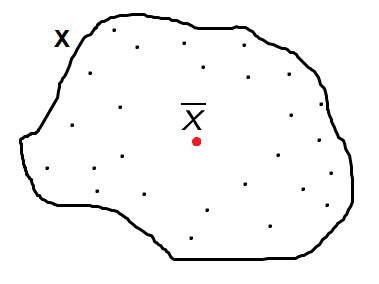
\includegraphics[scale=.8]{figuras/medida}
\end{figure}
\end{enumerate}
\inic Observe que nenhum dos dados são exatamente a média, porém todos estão em torno da média. Dizemos também, que uma média é bem representativa se todos os números desse banco de dados forem substituídos por $\overline{x}$, uma certa peculiaridade, por exemplo, soma ou produto dos números, será mantida. 

\subsection{Média para dados tabelados}
Como já vimos, dados tabelados são colocados em distribuição de frequência, considere o banco de dados $X_f=\{(x_1,f_i);(x_2,f_2);(x_3,f_3) \cdots, (x_n,f_n)\}$, sendo cada $x_i$ com sua respectiva frequência, logo a média aritmética é dada por

\begin{equation}
\label{tabelados}
    \overline{x} = \dfrac{\displaystyle\sum_{i=1}^{n}x_if_i}{\displaystyle\sum_{i=1}^nf_i} = \dfrac{x_1f_1 + x_2f_2 + x_3f_3 + \cdots + x_nf_n}{f_1 + f_2 + f_3 + \cdots + f_n},
\end{equation}
isto é, multiplicamos cada valor pela sua frequência e dividir pelo total de dados, ou seja, a soma das frequências.

\noindent \exemplo
\begin{enumerate}
    \item [(i)] Dada as distribuição de frequência, calcule a média aritmética
    \begin{table}[H]
        \caption{Distribuição de frequência }
        \centering
        \label{distri1}
        \begin{tabular}{cc}
        \hline
        $x_i$ & $f_i$ \\
        \hline
        2 & 10 \\
        3 & 5 \\
        4 & 12 \\
        6 & 11 \\
        \hline
    \end{tabular}
\end{table}
\inic Podemos fazer de duas formas, esteticamente falando, esse cálculo uma é usar diretamente a expressão \ref{tabelados}, que nos dá
\begin{align*}
    \overline{x} = \dfrac{2.10 + 3.5 + 4.12+6.11}{10+5+12+11} = 3,9210,
\end{align*}
a outra forma de realizar esta operação é criando novas colunas na Tabela \ref{distri1}, logo
\begin{table}[H]
        \centering
        \label{distri2}
        \begin{tabular}{ccc}
        \hline
        $x_i$ & $f_i$ & $x_if_i$ \\
        \hline
        2 & 10 & 20\\
        3 & 5 & 15\\
        4 & 12 & 48\\
        6 & 11 & 66\\
        \hline
        $\Sigma$ & 38 & 149
    \end{tabular}
\end{table}
\inic Basta agora dividirmos $149/38 = 3,9210$ .É importante frisar que, quando temos valores muitos diferentes dos demais, chamados valores aberrantes ou extremos, que não devemos utilizar a média aritmética para representa-los, pois esta é fortemente influenciada. Note pelo exemplo (ii)
\item [(ii)] Dada as distribuição de frequência, calcule a média aritmética
    \begin{table}[H]
        \caption{Distribuição de frequência }
        \centering
        \label{distri2}
        \begin{tabular}{cc}
        \hline
        $x_i$ & $f_i$ \\
        \hline
        2 & 10 \\
        3 & 5 \\
        4 & 12 \\
        6 & 11 \\
        1000 & 1\\
        \hline
    \end{tabular}
\end{table}
\begin{align*}
    \overline{x} = \dfrac{2.10 + 3.5 + 4.12+6.11+ 1000.1}{10+5+12+11+1} = 29,46,
\end{align*}
perceba que a média $29,46$ não representa bem os dados, pois a maioria destes estão abaixo de $10$ por exemplo.
\end{enumerate}
\subsection{Média ponderada}
Sejam os número reais $\{\omega_1, \omega_2,\omega_3,\cdots, \omega_n$\}. Quando queremos dar importância a mais para um tipo de dado do banco utilizamos a média ponderada, e chamamos cada $\omega_i$ de peso. definimos média ponderada por
\begin{equation}
    \label{peso}
    \overline{x} = \dfrac{\displaystyle\sum_{i=1}^{n}x_i\omega_i}{\displaystyle\sum_{i=1}^n\omega_i} = \dfrac{x_1\omega_1 + x_2\omega_2 + x_3\omega_3 + \dots + x_n\omega_n}{\omega_1 + \omega_2 + \omega_3 + \cdots + p_n},
\end{equation}
note que a média ponderada é uma generalização da média para dados tabelados, tento em vista que cada $f_i \in \mathbb{N}$ e cada $\omega_i \in \mathbb{R}$ sendo $\mathbb{N}\subset \mathbb{R}$.

\noindent \exemplo
\begin{enumerate}
    \item [(i)] Uma empresa de comunicação conta com 4 categorias de funcionários: Recepcionistas, Motoristas, Telemarketing e Diretoria. Os funcionários da primeira categoria recebem R\$ 950,35 mensalmente, segunda ganha R\$1.100,35 a terceira R\$ 1.111,21 enquanto os da quarta recebem R\$ 9501,53. Sabendo que essa empresa possui 63 funcionários no setor de telemarketing, 5 diretores, 4 motoristas e 12 recepcionistas, qual o salário médio pago por essa empresa? 
    \begin{align*}
        \overline{x} &= \dfrac{\displaystyle\sum_{i=1}^{4}x_i\omega_i}{\displaystyle\sum_{i=1}^4\omega_i} = \dfrac{x_1\omega_1 + x_2\omega_2 + x_3\omega_3+ x_4\omega_4}{\omega_1 + \omega_2 + \omega_3 + \omega_4}\\
        &= \dfrac{12.950,35 + 4.1100,35 + 63.1111,21 + 4.9501,53}{5 + 4 + 12 + 63} = 1474,02,
    \end{align*}
    \item[(ii)] (UNIUBE MG/2014) Um aluno deve atingir 70 pontos para ser aprovado. Esse total de pontos é resultado de uma média ponderada de 3 notas, $N_1$, $N_2$ e $N_3$, cujos pesos são, respectivamente, 1, 2, 2. As suas notas, $N_1$ e $N_2$, são, respectivamente, em um total de 100 pontos distribuídos em cada uma, 50 e 65. Para ser aprovado qual a nota $N_3$ numa escalade 0 a 100? 
    
    Neste problema temos a média o qual queremos atingir $\overline{x}=70$, e nos sobrará apenas os valor de $N_3$ logo, temos
    \begin{align*}
        70 &= \dfrac{1.50+2.65+2.N_3}{5}\\
        350 &= 2N_3 + 180 \\
        N_3&=85
    \end{align*}
\end{enumerate}

\subsection{Média em Intervalos de Classe}
\inic Para o cálculo da média quando os dados são contínuos, isto é, estão tabulados em intervalos de classe, basta definimos o ponto $p_i$ que é o ponto médio do intervalo da classe ($\ell_i$ = limite inferior do intervalo, $\ell_s$ = limite superior do intervalo) de calcularmos uma média para dado tabulados, levando em consideração o centro do intervalo, ou seja, sejam $n$ intervalos de classe, cada um com frequência $f_i$, então
\begin{equation}
    \overline{x} = \dfrac{\sum^{n}_{i=1}x_ip_i}{\sum^{n}_{i=1}p_i}
\end{equation}
Com $p_i = \dfrac{\ell_i + \ell_s}{2}$. 
\subsection{Média Geral}
\inic Sejam $\overline{x}_1, \overline{x}_2, \overline{x}_3, \cdots, \overline{x}_k$ as médias de $k$ séries de dados, com $n_1,n_2,n_3, \cdots, n_k$ o número de termos de cada série. Chamamos média geral, denotada por $\overline{x}^{(g)}$ a expressão
\begin{equation}
    \overline{x}^{(g)} =  \frac{\displaystyle\sum_{i=1}^{n}\overline{x}_in_i}{\displaystyle\sum_{i=1}^{n}n_i} = \frac{n_1\overline{x}_1 + n_2\overline{x}_2 + n_3\overline{x}_3 + \cdots + n_k\overline{x}_k}{n_1 + n_2 + n_3 +  \cdots, + n_k},
\end{equation}
em suma, para calcular uma média geral, você precisa ter $k$ bancos de dados, suas médias e seus respectivos tamanhos. Basicamente, a média geral é também uma média ponderada usando como pesos a quantidade de indivíduos do banco de dados.

\begin{figure}[H]
    \label{mediaintgeo}
	\centering
	\caption{Média Geral}
	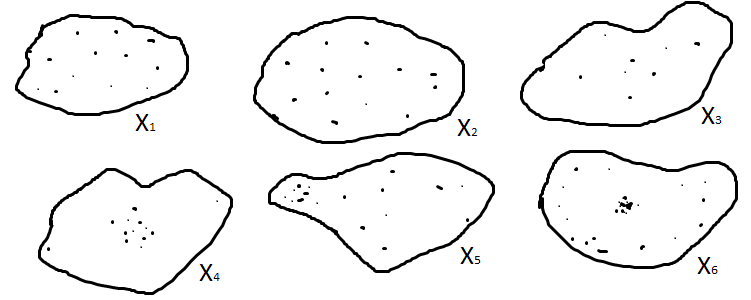
\includegraphics[scale=.8]{figuras/banco6}
\end{figure}

\noindent \exemplo
\begin{enumerate}
    \item [(i)] Considere o banco de dados com médias $\overline{x} = 10$ e $\overline{y} = 11,42$ sendo $\sum_{i=1}^{n}x_i=50$ e $\sum_{j=1}^{m}y_i=80$, calcule o número de elementos de cada população e a média geral.
    
    \inic Para calcular a média geral, basta determinarmos quantos indivíduos existem em cada população, de fato
    \begin{align*}
        \overline{x} = \frac{\sum_{i=1}^{n}x_i}{n_x} \Rightarrow n_x = \frac{\sum_{i=1}^{n}x_i}{\overline{x}} \Rightarrow n_x = \frac{50}{10} = 5\\
         n_y = \frac{\sum_{j=1}^{m}y_j}{\overline{y}} \Rightarrow n_y = \frac{80}{11,42} \approx 7 
    \end{align*}
    Agora basta calculamos a média geral, temos
    \begin{align*}
        \overline{x}^{(g)} = \frac{\overline{x}n_x + \overline{y}n_y}{n_x+n_y} = \frac{10.5+11,42.7}{5+7} = \frac{20}{3}
    \end{align*}
    
    \item[(ii)] Em uma empresa a média de idade das mulheres é $\overline{M} = 28$ e dos homens é $\overline{H} = 32$, sabe-se que somando as idades de todos os homens temos $544$, e se somarmos a idade das mulheres temos $644$. Determine a média de idade dos funcionários dessa empresa.
    
    \inic Temos um problema parecido com o anterior, com a diferença o contexto que não pede de maneira explícita o cálculo da média geral, de fato, vamos calcular primeiramente quantos homens e quantas mulheres há nesta empresa.  
    \begin{align*}
    n_M &= \frac{644}{28} = 23, \\
    n_H &= \frac{544}{32} = 17.
    \end{align*}
    \inic Agora, calculamos a média geral, logo
    \begin{equation*}
        \overline{x}^{(g)} = \frac{\overline{H}n_H + \overline{M}n_M}{n_H+n_M} = \frac{32.17 + 28.23}{23+17} = 29,7.
    \end{equation*}
    
\end{enumerate}

\subsection{Outras Médias}
\subsubsection{Média Geométrica}
Considere novamente o banco de dados $X$ associados ao conjunto de frequências $F$, a média geométrica $\overline{x}_g$ é definida por

\begin{equation}
    \overline{x}_g = \sqrt[n]{\prod_{i=1}^nx_i} = \sqrt[n]{x_1x_2x_3\cdots x_n}.
\end{equation}
\inic A média geométrica possui aplicações em diversas áreas da ciência, uma das aplicações mais usuais é no mercado financeiro, ao invés de calcularmos a média arimética, usamos a geométrica para cálculos de taxas médias.
Seja o banco de dados $\mathnormal{X}= \{\mathnormal{x}_1,\mathnormal{x}_2,\mathnormal{x}_3,\cdots, \mathnormal{x_n}\}$ com $\mathnormal{n}$ elementos, e suas respectivas frequências $\mathnormal{F} = \{\mathnormal{f}_1,\mathnormal{f}_2,\cdots,\mathnormal{f_n}\}$, assim calculamos:


\begin{equation}
	\overline{\mathnormal{x}}_{\mathnormal{g}} = \sqrt[\mathnormal{n}]{\mathnormal{x}_1^{\mathnormal{f}_1}\mathnormal{x}_2^{\mathnormal{f}_2}\mathnormal{x}_3^{\mathnormal{f}_3}\cdots \mathnormal{x_n}^{\mathnormal{f_n}}}
\end{equation}
em alguns momentos será necessário o cálculo de $\log \mathnormal{\overline{x}_g}$ pela expressão:
\begin{equation*}
	\log \overline{x}_g = \dfrac{\displaystyle\sum_{i=1}^{n} f_i \log x_i}{n} = \frac{f_1 \log x_1 + \cdots + f_n \log x_n}{n}
\end{equation*}

\noindent \exemplo
\begin{enumerate}
	\item[(i)] Calcule a média geométrica dos dados abaixo:
		\begin{enumerate}
			\item[(a)] 3 - 6 - 12 - 24 - 48;
			\item[(b)] \begin{tabular}{ll}
				\hline
				$\mathnormal{x_i}$ & $\mathnormal{f_i}$\\
				\hline
				1 & 8 \\
				2 & 6 \\
				3 & 5 \\
				5 & 3 \\
				\hline
			\end{tabular}
		\end{enumerate}
		%\item[(ii)]
	\end{enumerate}

\subsubsection{Média Harmônica}
Os comentários e exemplos aqui citados, foram retirados de \cite{hariki1996media}.

Um número $\overline{x}_H$ é a média harmônica de um conjunto de banco de dados $X$ se 
\begin{align}
    \label{harmonica}
    \frac{1}{x_1} + \frac{1}{x_2} + \frac{1}{x_3} + \cdots + \frac{1}{x_n} &= \underbrace{\frac{1}{\overline{x}_H} + \frac{1}{\overline{x}_H} + \frac{1}{\overline{x}_H} + \cdots + \frac{1}{\overline{x}_H}}_{n},\\
    \label{harmonica2}
    \frac{1}{x_1} + \frac{1}{x_2} + \frac{1}{x_3} + \cdots + \frac{1}{x_n} &= \frac{n}{\overline{x}_H},\\ 
    \label{harmonica3}
    \overline{x}_H &= \frac{n}{\frac{1}{x_1} + \frac{1}{x_2} + \frac{1}{x_3} + \cdots + \frac{1}{x_n}}
\end{align}
Para dados agrupados temos 
\begin{equation}
    \overline{x}_H = \frac{f_1 + f_2 + f_3 + \cdots + f_n}{\frac{f_1}{x_1} + \frac{f_2}{x_2} + \frac{f_3}{x_3} + \cdots + \frac{f_n}{x_n}},
\end{equation}
a ideia de média harmônica aparece quanto pretendemos calcular uma média entre razões de grandezas sendo a grandeza do numerador é a mesma dentro do problema específico. 

\noindent \exemplo
\begin{enumerate}
    \item [(i)] Determine a média harmônica entre 2, 5, 8.
    Basta aplicarmos a expressão \ref{harmonica3}, para $n=3$, logo
    \begin{align*}
        \overline{x}_H = \frac{3}{\frac{1}{2} + \frac{1}{5} + \frac{1}{8}} = 3,64
    \end{align*}
    \item[(ii)] Um motorista vai de Recife a Caruaru com uma velocidade média de $80 km/h$. Chegando lá, retorna, utilizando o mesmo percurso, para o local onde partiu em Recife, com velocidade de média de $100 km/h$. Qual a velocidade média do percurso? 
    
    \inic Note que no problema queremos a média da razão \textit{deslocamento}/\textit{tempo}, na qual o deslocamento é o mesmo para as duas razões. Então tome $d$ deslocamento, $t_i$ o tempo de ida, $t_v$ o tempo de volta e $V$ a velocidade média, logo
    \begin{align*}
        V&= \frac{2d}{t_i + t_v}\Rightarrow t_i + t_v = \frac{2d}{V},\,\, \text{como}\,\, t_i = \frac{d}{80}\,\, \text{e}\,\, t_v = \frac{d}{100}\\
        \frac{2}{V} &= \frac{1}{80} + \frac{1}{100} \Rightarrow V \approx 88,9 km/h
    \end{align*}
    \item[(iii)] Um grande tanque possui três torneiras. A torneira A enche o tanque em 4h, a B, em 3h e a C em 6h. Deseja-se substituí-las por três torneiras idênticas, de modo que essas três novas ligadas simultaneamente encham o tanque no mesmo tempo que as torneiras A, B e C ligadas juntas. Quanto tempo será necessário par apenas umas dessas novas torneiras encher o tanque? 
    
    \inic Aqui tomaremos o tempo unitário, isto é, em 1h vemos que a torneira $A$ enche $1/4$ do tanque, a $B,\,\,1/3$ e a $C,\,\,1/6$. Digamos que as torneiras novas encham, sozinhas, cada uma o tanque em $T$ horas. Logo, cada uma, em 1h encherá $1/T$ do tanque. Portanto, em uma hora a fração do tanque que estará cheia será: 
    \begin{align*}
        \frac{3}{T} &= \frac{1}{4} + \frac{1}{3} + \frac{1}{6},\\
        T&=4.
    \end{align*}
\end{enumerate}

\section{Medidas de Posição}
\subsection{Mediana}

\begin{defin}
Sejam um banco de dados $X = \{x_1,x_2,x_3,\cdots, x_n\}$, definimos mediana, denotado por $\Tilde{x}$, o valor numérico que divide a série de dados em duas partes de tamanhos iguais.
\end{defin}
Geometricamente, em uma dimensão, podemos representar a medida por

\begin{figure}[H]
	\centering
	\caption{Interpretação geométrica da Mediana}
	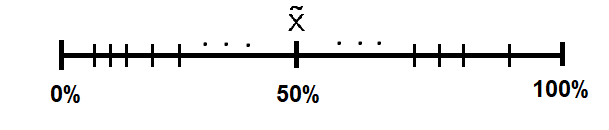
\includegraphics[scale=.9]{figuras/mediana.png}
\end{figure}
Importante frisar que a mediana é uma medida que não é afetada por valores extremos. Para determinar posição da mediana, em dados discretos, temos dois casos:
	\begin{equation}
	\label{medianadis}
		\Tilde{x} = \begin{cases}
		\mathnormal{x}_{\left(\frac{\mathnormal{n}+1}{2}\right)}, \, \text{se}\,\, \mathnormal{n}\,\,\text{é impar}\\
		\\
		\dfrac{\mathnormal{x}_{\left(\frac{\mathnormal{n}}{2}\right)}+\mathnormal{x}_{\left(\frac{\mathnormal{n}}{2}+1\right)}}{2}, \,\,\text{se}\,\, \mathnormal{n}\,\,\text{é par}
		\end{cases}
	\end{equation}	
para calcular a mediana para dados contínuos, ou seja, tabulados em intervalos de classe temos os seguintes passos

\begin{enumerate}
    \item[(i)] Calcula-se a ordem $n/2$, sendo $N = \sum f_i$;
    \item[(ii)] Use a $f_{ac}$ para identificar a classe mediana;
    \item[(iii)] Utiliza-se a fórmula:
    \begin{equation}
    \label{medianacont}
    \tilde{x} = \ell_{\tilde{x}} + \frac{\left(\dfrac{N}{2}-\sum f_i\right)h}{f_{\tilde{x}}}
    \end{equation}
\end{enumerate}
sendo
\begin{itemize}
     \item $\ell_{\tilde{x}}$: limite inferior da classe mediana;
     \item $N$: número de elementos;
     \item $\sum f$: soma das frequências anteriores à classe mediana;
     \item $h$: amplitude da classe mediana;
     \item $f_{\tilde{x}}$: frequência da classe mediana.
\end{itemize}

\noindent \exemplo
\begin{enumerate}
    \item[(i)] Calcule a mediana dos dados abaixo:
    \begin{enumerate}
        \item[(a)] 8 - 5 - 8 - 10 - 8 - 9 - 10 - 9 - 12 - 13 - 20 - 30 - 40;
        \item[(b)] 
        \begin{center}
        \begin{tabular}{cc}
            \hline
            $x_i$ & $f_i$ \\
            \hline
            2  & 4  \\
            4  & 8  \\
            8  & 16 \\
            16 & 32 \\
            32 & 64 \\
            \hline
        \end{tabular}
        \end{center}

        \item[(c)] 
        \begin{center}
        \begin{tabular}{cc}
            \hline
            $x_i$ (classe) & $f_i$ \\
            \hline
            35 $\vdash$ 45 & 5  \\
            45 $\vdash$ 55 & 12 \\
            55 $\vdash$ 65 & 18 \\
            65 $\vdash$ 75 & 14 \\
            75 $\vdash$ 85 & 6  \\
            85 $\vdash\hspace{-0.2cm}\dashv$ 95 & 3 \\
            \hline
        \end{tabular}
        \end{center}
    \end{enumerate}
\end{enumerate}

\inic O item (a) basta colocarmos os dados em ordem crescente identificarmos a paridade de $n$, logo\\

\begin{center}
 5 - 8 - 8 - 8 - 8 - 9 - 9 - 9 - 10 - 10 - 12 - 13 - 20 - 30 - 40   
\end{center}
 como temos $ n = 15$, logo usando a expressão (\ref{medianadis}), temos
 $$
 \Tilde{x} = x_{\left(\frac{n+1}{2}\right)} = x_{\left(\frac{15+1}{2}\right)} = x_{(8)}
 $$
isto é, a mediana será o elemento $x_{(8)} = 9$.

\inic Para o item (b), basta identificarmos a também onde se localiza $\sum f_i/2$, isto é, $\sum f_i/2 = 124/2 = 62$ e agora construimos a coluna de frequências acumuladas, logo

\begin{table}[H]
    \centering
    \begin{tabular}{ccc}
	\hline
	$x_i$ & $f_i$ & $f_{ac}$\\
	\hline
	2 & 4 & 4\\
	4 & 8 & 12\\
	8 & 16 & 28\\
	16 & 32 & 60\\
	32 & 64 & 124\\
	\hline
    \end{tabular}
\end{table}
\inic Logo a mediana será o dado cuja frequência ultrapassou $\sum f_i/2 = 62$, isto é, $\Tilde{x} = 32$.

\inic Para o item (c) usaremos (\ref{medianacont}) e seguiremos os passos dados, assim 
\begin{table}[H]
    \centering
    \begin{tabular}{ccc}
	    \hline
	    $x_i$ & $f_i$ & $f_{ac}$\\
	    \hline
	    35 $\vdash$ 45 & 5 & 5\\
        45 $\vdash$ 55 & 12 & 17\\
	    55 $\vdash$ 65 & 18 & 35\\
        65 $\vdash$ 75 & 14 & 49\\
	    75 $\vdash$ 85 & 6 & 55\\
	    85 $\vdash \hspace{-0.2 cm }\dashv$ 95 & 3 & 58\\
	    \hline
    \end{tabular}
\end{table}

\inic Logo pelo critério do item (b)  definimos a classe que contém a mediana como sendo $55 \vdash 65$ e assim

\begin{equation*}
    \begin{cases}   
        \ell_{\Tilde{x}} = 55\\
        N/2 = 29\\
        \sum f_i = 17\\
        h = 65-55 = 10\\
        f_{\Tilde{x}} = 18,
    \end{cases}
\end{equation*}
Agora basta substituir em (\ref{medianacont}), temos

\begin{align*}
    \tilde{x} &= \ell_{\tilde{x}} + \frac{\left(\dfrac{N}{2} - \sum f_i \right) h}{f_{\tilde{x}}} \\
    &= 55 + \frac{(29 - 17) \cdot 10}{18} \approx 61{,}67
\end{align*}



\subsection{Quartis}
\inic Seja o banco de dados $X$ organizados em rol, definem-se \textit{quartis} os valores da distribuição que dividem o banco de dados em quatro partes iguais, isto é:

	\begin{figure}[H]
		\centering
		\caption{Forma geométrica dos quartis em uma dimensão}
		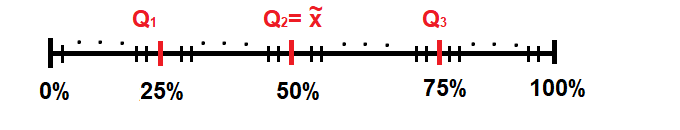
\includegraphics[scale=.8]{figuras/quartis.png}
	\end{figure}
	
	Como $Q_2 = \tilde{x}$, para calcular $Q_1$ e $Q_3$, temos:
\begin{equation}
    \label{quartis}
    Q_i = \ell_{Q_i} + \dfrac{\left(\dfrac{in}{4} - \sum f_i \right) h}{f_{Q_i}}.
\end{equation}

\begin{itemize}
    \item $\ell_{Q_i}$: limite inferior da classe do quartil;
    \item $\sum f$: soma das frequências anteriores à classe do quartil;
    \item $h$: amplitude da classe do quartil;
    \item $f_{Q_i}$: frequência da classe do quartil.
\end{itemize}

\noindent \exemplo

\subsection{Decis}

\inic Agora $X$ será organizado em rol. Definem-se \textit{decis} os valores da distribuição que dividem o banco de dados em dez partes iguais, isto é:
\begin{figure}[H]
    \centering
    \caption{Interpretação geométrica dos Decis em uma dimensão}
    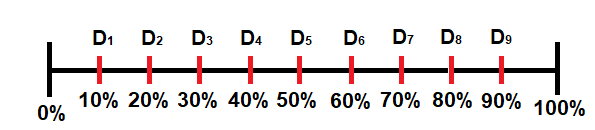
\includegraphics[scale=.7]{figuras/decil}
\end{figure}

Como $D_5 = \tilde{x}$, para calcular os demais, temos:
\begin{equation}
\label{decil}
D_i = \ell_{D_i} + \dfrac{\left(\dfrac{in}{10} - \sum f_i \right) h}{f_{D_i}}.
\end{equation}

\begin{itemize}
    \item $\ell_{D_i}$: limite inferior da classe do decil;
    \item $\sum f$: soma das frequências anteriores à classe do decil;
    \item $h$: amplitude
\end{itemize}

\subsection{Percentis}

\inic Seja $X$ organizado em rol. Definem-se \textit{percentis} os valores da distribuição que dividem o banco de dados em cem partes iguais, isto é:
\begin{figure}[H]
    \centering
    \caption{Interpretação geométrica dos Percentis em uma dimensão}
    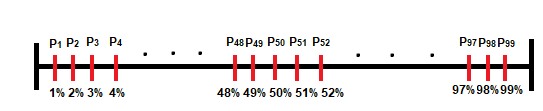
\includegraphics[scale=.7]{figuras/percentil}
\end{figure}

Como $P_{50} = \tilde{x}$, para calcular os demais, temos:
\begin{equation}
\label{percentil}
P_i = \ell_{P_i} + \dfrac{\left(\dfrac{in}{100} - \sum f_i \right) h}{f_{P_i}}.
\end{equation}

\begin{itemize}
    \item $\ell_{P_i}$: limite inferior da classe do percentil;
    \item $\sum f$: soma das frequências anteriores à classe do percentil;
    \item $h$: amplitude da classe do percentil;
    \item $f_{P_i}$
\end{itemize}
\inic O uso das fórmulas (\ref{quartis}), (\ref{decil}) e (\ref{percentil}) são todos semelhantes à (\ref{medianacont}), e podem ser perfeitamente aplicados a dados de exemplos anteriores.
Um esquema importante é o \textit{Esquema dos cinco números}. este procura estabelece as cinco principais estatísticas de ordem existentes que são: $x_{(1)}, x_{(n)}, Q_1, Q_3, Md$, isto é, mínimo, máximo, 25\% dos dados 50\% dos dados e 75\% dos dados. 


\subsection{Box plot}
\inic O \textit{box plot} é um gráfico que dá a ideia da posição, dispersão, assimetria, caudas e dados discrepantes, em geral é usado para analisar geometricamente as medidas de posição, temos

\begin{figure}[H]
	\centering
	\caption{Boxplot}
	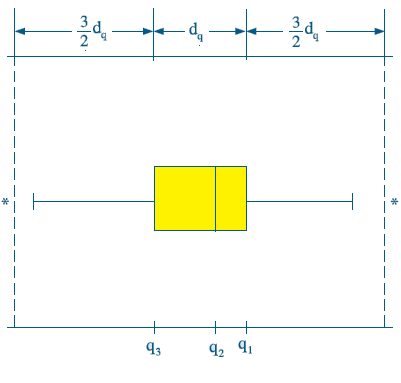
\includegraphics[scale=.6]{figuras/box.png}
	\begin{center}
	Fonte: \cite{morettin2017estatistica}
	\end{center}
\end{figure}

Para o cálculo dos elementos do \textit{Boxplot}, isto é, limites superior ($L_S$) e inferior ($L_I$) temos:
	\begin{equation}
		\begin{cases}
		    L_I = \max\{\min\{x_i\}, Q_1-1,5(Q_3-Q_1)\}\\
		    L_S = \min\{\max\{x_i\}, Q_1+1,5(Q_3-Q_1)\}
		\end{cases}
	\end{equation}

Para construir um \textbf{boxplot} no \textit{Rstudio} usaremos o comando \textbf{boxplot()}, que possui os seguintes argumentos básicos:
\begin{enumerate}
	\item[(i)] $x$ é o vetor de dados;
	\item[(ii)] ``main =" é o título do gráfico;
	\item[(iii)] ``xlab = "\, é o texto no eixo x;
	\item[(iv)] ``ylab = "\, é o texto no eixo y;
	\item[(v)] ``col ="\, é a cor do preenchimento da caixa;
	\item[(vi)] ``border ="\, cor da linha da borda da caixa; 
	\item[(vii)] ``horizontal ="\, se \textbf{TRUE} o gráfico ficará na horizontal, se \textbf{FALSE} ficará na vertical.
\end{enumerate}
\inic Outra importante ferramente é o comando ``fivenum(x, na.rm = TRUE)", que dá os 5 número representativos do boxplot.

\section{Moda ($M_o$)}
\inic Seja o banco de dados $\mathnormal{X}= \{\mathnormal{x}_1,\mathnormal{x}_2,\mathnormal{x}_3,\cdots, \mathnormal{x_n}\}$ com $\mathnormal{n}$ elementos, e suas respectivas frequências $\mathnormal{F}=\{\mathnormal{f}_1,\mathnormal{f}_2,\cdots,\mathnormal{f_n}\}$, definimos \textit{Moda} o valor de $\mathnormal{x_i}$ que possui maior frequência, isto é, seja o par $(\mathnormal{x_i,f_i})$ temos:
	\begin{equation*}
		Mo = \{\mathnormal{x_i} \in \mathbb{R}/ (\mathnormal{x_i}, max\{\mathnormal{f_1},\cdots,\mathnormal{f_n}\})\},
	\end{equation*}
para moda de dados discretos basta observamos a que possui maior $f_i$. Para dados em intervalos de classe temo a fórmula de Czuber, a qual seguiremos os seguinte passos
\begin{enumerate}
        \item[(i)] Identifica-se a classe modal;
		\item[(ii)] Usa-se a fórmula;
		\begin{equation}
		\label{Czuber}
		\mathnormal{Mo} = \ell_{Mo} + \frac{\mathnormal{\Delta}_1}{\mathnormal{\Delta}_1 + \mathnormal{\Delta}_2}\mathnormal{h},
		\end{equation}
	\end{enumerate}
	sendo:
	\begin{itemize}
		\item $\ell_{Mo}$: limite inferior da classe modal;
		\item $\mathnormal{\Delta}_1$: Diferença entre a frequência da classe modal e a imediatamente anterior;
		\item $\mathnormal{\Delta}_2$: Diferença entre a frequência da classe modal e a imediatamente posterior;
		\item $\mathnormal{h}$: amplitude da classe modal.
	\end{itemize}

\exemplo
\begin{enumerate}
    \item[(i)] Calcule a moda dos dados abaixo:
	\begin{enumerate}
	    \item[(a)] 8 - 5 - 8 - 10 - 8 - 9 - 10 - 9 - 12 -13 - 20 - 30 - 40;
		\item[(b)] \begin{tabular}{cc}
	    	\hline
			$\mathnormal{x_i}$ & $\mathnormal{f_i}$\\
			\hline
			2 & 4 \\
			4 & 8 \\
			8 & 16 \\
			16 & 32 \\
			32 & 64 \\
			\hline
		\end{tabular}
		\qquad \qquad (c) \begin{tabular}{cc}
			\hline
			$\mathnormal{x_i}$ & $\mathnormal{f_i}$\\
			\hline
			35 $\vdash$ 45 & 5\\
			45 $\vdash$ 55 & 12\\
			55 $\vdash$ 65 & 18\\
			65 $\vdash$ 75 & 14\\
			75 $\vdash$ 85 & 6\\
			85 $\vdash \hspace{-0.2 cm }\dashv$ 95 & 3\\
			\hline
		\end{tabular}
	\end{enumerate}
\end{enumerate}

\inic No Item (a) basta contarmos quais elementos aparecem mais, daí note que $M_o = 8$. Para o item (b) basta olharmos a coluna de frequências absolutas, note que a maior é do dado $x_i = 32$, logo $M_o = 32$. Para o item (c) aplicaremos os passos da fórmula de Czuber, logo \begin{equation*}
    \begin{cases}
        \mathtt{l}_{Mo} = 55\\
        \Delta_1 = 18-12 = 6\\
        \Delta_2 = 18- 14 = 4\\
        h = 10
    \end{cases}
\end{equation*}


\begin{align*}
    \mathnormal{Mo} &= \ell_{Mo} + \frac{\mathnormal{\Delta}_1}{\mathnormal{\Delta}_1 + \mathnormal{\Delta}_2}\mathnormal{h} = 55 + \frac{6}{6+4}10\\
    &= 61
\end{align*}
\inic Uma observação importante é que nem toda a série de dados possui apenas uma moda, poderíamos ter, por exemplo, um banco $X = \{2,2,3,3,4,5,6,7\}$, ou seja,um banco que possui duas modas, o que chamamos de \textit{série bimodal}, bem como temos com $3,4,\cdots, n$ modas, que são as séries $n$-modais. Se a série não possuir moda chamamos de \textit{Amodal}, por exemplo $Y = \{1,1,2,2,3,3,4,4,5,5\}$ 

\section{Medidas de Dispersão}
\inic São medidas que têm o objetivo de mensurar o afastamento dos dados de suas medidas de tendência central, em geral a média. Observe que na Figura há dois bancos de dados, que possuem a mesma média porém o dados não se comportam de maneira semelhante.

\begin{figure}[H]
	\centering
	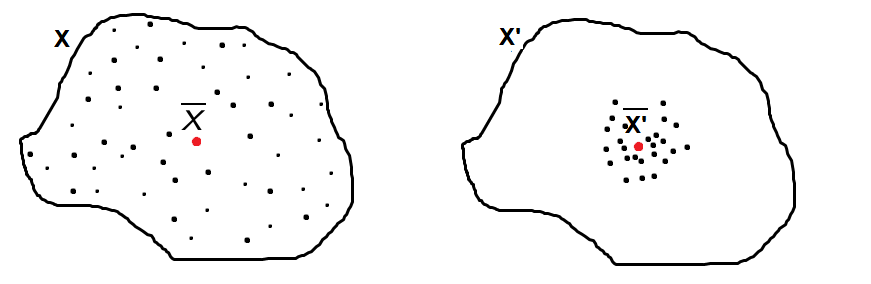
\includegraphics[scale=.65]{figuras/dispersao}
\end{figure}
\inic Note que em $X'$ os dados estão mais concentrados em torno da média, o que não ocorre com tanta evidência em $X$. Daremos agora um exemplo numérico da da situação explorada.

\noindent\exemplo\\
Sejam os bancos de dados $\mathnormal{X}=\{40,40,40,40,40,40,40\}$ e $\mathnormal{Y}=\{40, 60, 10,30,100,0,50,30\}$, note que $\mathnormal{\overline{x}} = \mathnormal{\overline{y}}= 40$, porém os bancos não possuem o mesmo comportamento, enquanto todos os valores de $X$ são exatamente iguais a média, os demais estão a uma certa distância não nula. Em estatística não podemos dizer que um banco de dados como $X$ e $Y$ são iguais, para diferenciar esses bancos de dados defini-se as \textit{medidas de dispersão}.

\subsection{Desvio}
\inic Seja o banco de dados $\mathnormal{X}$ com $\mathnormal{n}$ elementos e média $\mathnormal{\overline{x}}$ definimos desvio em relação ao dado $\mathnormal{x_i}$, denotado por $\mathnormal{D_i}$,  com $\mathnormal{i}=1,2,3,\cdots,\mathnormal{n}$ tal que:

\begin{equation}
	\mathnormal{D_i} = \mathnormal{x_i} - \mathnormal{\overline{x}}.	
\end{equation}
\inic Pelo fato termos indexado os desvios, cada dado terá o seu, de fato, observe o banco de dados do exemplo. 

\noindent \exemplo 

\begin{enumerate}
    \item [(i)] Determine os $D_i's$ do banco $X = \{5,2,3,4,5,5,6,10\}$.
    Primeiramente, vamos calcular a média deste banco de dados, temos 
    \begin{align*}
        \overline{x} = \dfrac{5 + 2 + 3 + 4 + 5 + 5 + 6 + 10}{8} = 5
    \end{align*}
\end{enumerate}
Agora, calcularemos os desvios dos dados, nesta ordem, $X = \{x_1 = 5,x_2 = 2,\cdots, x_8 = 10\}$ logo
\begin{equation*}
    \begin{cases}
    D_1 = x_1 - \overline{x} = 5 - 5 =0\\
    D_2 = x_2 - \overline{x} = 2 - 5 =-3\\
    D_3 = x_3 - \overline{x} = 3 - 5 =-2\\
    D_4 = x_4 - \overline{x} = 4 - 5 =-1\\
    D_5 = x_5 - \overline{x} = 5 - 5 =0\\
    D_6 = x_6 - \overline{x} = 5 - 5 =0\\
    D_7 = x_7 - \overline{x} = 6 - 5 =1\\
    D_8 = x_8 - \overline{x} = 10 - 5 =5
    \end{cases}
\end{equation*}
\begin{prop}
\label{desvios0}
A soma dos desvios é igual a zero.
\end{prop}

\begin{proof}
Considere o banco de dados $X = \{x_1,x_2,x_3,\cdots,x_n\}$ sendo que cada $x_i$ pode ser contínuo ou discreto. Então temos
\begin{align}
    \label{p1}
    D_i &= x_i - \overline{x}\\ 
    \label{p2}
    \sum_{i=1}^{n} D_i &= \sum_{i=1}^{n} (x_i - \overline{x})\\
    \label{p3}
      &= \sum_{i=1}^{n} x_i - n\overline{x}
\end{align}
mas pela definição de média temos $\overline{x} = \sum_{i=1}^{n} x_i/n \Rightarrow n\overline{x} = \sum_{i=1}^{n} x_i$ que substituindo em (\ref{p3}) concluímos a demonstração.
\end{proof}

\subsection{Desvio Médio}
No banco de dados $\mathnormal{X}$ com $\mathnormal{n}$ elementos e média $\overline{x}$, definimos \textit{desvio médio}, denotado por $\mathnormal{D_M}$ a expressão:
\begin{equation}
	D_M = \frac{\displaystyle \sum_{i=1}^{n}|x_i-\overline{x}|}{n},
	\end{equation}
para dados agrupados temos:
\begin{equation}
	D_M = \frac{\displaystyle \displaystyle \sum_{i=1}^{n} |x_i-\overline{x}|f_i}{n}
\end{equation}
Por exemplo, vamos calcular os desvio médio dos dados do exemplo da subseção de desvios, isto é, o conjunto $X = \{x_1 = 5,x_2 = 2,\cdots, x_8 = 10\}$, onde temos o conjunto de desvios $D = \{D_1 = 0, D_2 = -3, D_3 = -2, D_4 = -1, D_5 = 0, D_6 = 0, D_7 = 1, D_8 = 5\}$ agora calculando o desvio médio
\begin{align*}
    D_M &= \dfrac{\displaystyle \sum_{i=1}^{n} |D_i|}{n}\\
    &= \dfrac{|0| + |-3| + |-2| + |-1| + |0| + |0| + |1|+ |5|}{8}\\
    &= \dfrac{12}{8} = 1,5.
\end{align*}

\inic Isto é, em média os dados estão a uma distância de 1,5 da média. A definição de desvio médio é uma das soluções que foram encontradas para resolvermos o problema do cálculo de uma medida que represente a variação dos dados, tendo em vista o problema a Proposição \ref{desvios0}. Porém algumas propriedades de valor absoluto podem ser problema, por exemplo note que o valor absoluto não é uma função suave assim não pode-se derivar, para isso definiremos variância

\subsection{Variância}
\inic Outra forma de evitar que a soma dos desvio seja zero é considerando o quadrado da soma, assim definimos variância, denotada por $\sigma^2$ quando populacional e $s^2$ quando amostral, a expressão:
	\begin{equation}
	\label{var}
		\sigma^2 = \frac{\displaystyle \sum_{i=1}^{n} (x_i-\overline{x})^2}{n},
	\end{equation}
	para dados agrupados:
	\begin{equation}
	\label{varf}
		\sigma^2 = \frac{\displaystyle \sum_{i=1}^{n} (x_i-\overline{x})^2f_i}{\displaystyle\sum_{i=1}^{n} f_i}.
	\end{equation}

 \begin{defin}[Desvio Padrão]
    Definimos \textit{desvio padrão} por $\sigma = \sqrt{\sigma^2}$.
 \end{defin}
 
 \noindent \exemplo
 \begin{enumerate}
	\item[(i)] Nos dados abaixo, o desvio médio e o desvio padrão  de cada distribuição:
	\begin{enumerate}
		\item[(a)] 8 - 5 - 8 - 10 - 8 - 9;
		\item[(b)] \begin{tabular}{cc}
			\hline
			$x_i$ & $f_i$\\
			\hline
			5 & 2 \\
			6 & 3 \\
			8 & 5 \\
			9 & 32 \\
			11 & 64 \\
			\hline
		\end{tabular}
		\qquad \qquad \qquad (c) \begin{tabular}{cc}
			\hline
			$x_i$ & $f_i$\\
			\hline
			35 $\vdash$ 45 & 5\\
			45 $\vdash$ 55 & 12\\
			55 $\vdash$ 65 & 18\\
			65 $\vdash$ 75 & 14\\
			75 $\vdash$ 85 & 6\\
			85 $\vdash \hspace{-0.2 cm }\dashv$ 95 & 3\\
			\hline
		\end{tabular}
	\end{enumerate}
	Para solucionar o item (a) temos a aplicação da expressão (\ref{var}), para isso necessitamos da média, que será $\overline{x}=8$, logo o cálculo do desvio médio será
	\begin{align*}
	    D_M &= \frac{\displaystyle \sum_{i=1}^{6} |x_i-\overline{x}|}{n}\\
	     &= \dfrac{|x_1-\overline{x}| + |x_2-\overline{x}| + |x_3-\overline{x}| + |x_4-\overline{x}| + x_5-\overline{x}| + |x_6-\overline{x}|}{6}\\
	     &= \dfrac{|8-8| + |5-8| + |8-8| + |10-8| + |8-8| + |9-8|}{6}=\dfrac{6}{6}\\ 
	    &= 1
	\end{align*}
	e o desvio padrão
	\begin{align*}
	    \sigma^2 &= \frac{\displaystyle \sum_{i=1}^{6} (x_i-\overline{x})^2}{n}\\
	     &= \dfrac{(x_1-\overline{x})^2 + (x_2-\overline{x})^2 + (x_3-\overline{x})^2 + (x_4-\overline{x})^2 + (x_5-\overline{x})^2 + (x_6-\overline{x})^2}{6}\\
	     &= \dfrac{(8-8)^2 + (5-8)^2 + (8-8)^2 + (10-8)^2 + (8-8)^2 + (9-8)^2}{6}=\dfrac{14}{6}\\ 
	    &= 2,8,
	\end{align*}
	logo o desvio padrão será 
	\begin{equation*}
	    \sigma = \sqrt{\sigma^2} = \sqrt{2,8} = 1,6732
	\end{equation*}
\end{enumerate}
 No item (b) temos que $\overline{x} = 20$ e aplicaremos a expressão (\ref{varf}), logo
 \begin{align*}
	    \sigma^2 &= \frac{\displaystyle \sum_{i=1}^{5} (x_i-\overline{x})^2f_i}{\displaystyle\sum_{i=1}^{5}f_i}\\
	     &= \dfrac{(x_1-\overline{x})^2f_1 + (x_2-\overline{x})^2f_2 + (x_3-\overline{x})^2f_3 + (x_4-\overline{x})^2f_4 + (x_5-\overline{x})^2f_5}{f_1 + f_2 + f_3 + f_4 + f_5}\\
	     &= \dfrac{(5-20)^22 + (6-20)^23 + (8-20)^25 + (9-20)^232 + (11-20)^264}{106}=\dfrac{10814}{106}\\ 
	    &= 102,0188
	\end{align*}
\section{Assimetria e Curtose}
\subsection{Assimetria}
\inic Chamamos \textit{assimetria} o grau de afastamento de uma distribuição da unidade de simetria. Em uma distribuição simétrica tem-se a igualdade dos valores da média, mediana e moda, logo
\begin{figure}[H]
	\centering
	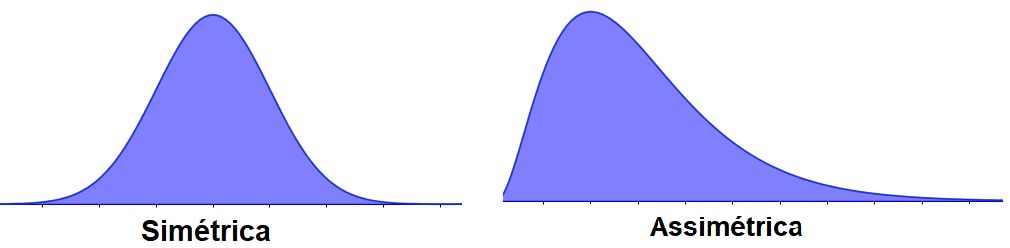
\includegraphics[scale=.5]{figuras/simetria}
\end{figure}
\noindent cujo temos por classificação, para uma distribuição unimodal:
	\begin{enumerate}
	    \item[(i)] \textbf{Simétrica}: se $Mo = Md = \overline{\mathnormal{x}}$;
		\item[(ii)] \textbf{Assimétrica positiva}: se $Mo < Md < \overline{\mathnormal{x}}$;
		\item[(iii)] \textbf{Assimétrica negativa}: se $\overline{\mathnormal{x}} < Md < Mo$.
	\end{enumerate}
\inic Para mensurar a simetria de uma distribuição este temos dois coeficientes, denominados 1º e 2º coeficientes de Pearson definidos por:

    \begin{equation}
	    AS = \frac{\overline{x} - Mo}{\sigma},
    \end{equation}
	ou
	\begin{equation}
	    AS = \frac{Q_1 + Q_3 - 2Md}{Q_3-Q_1}.
	\end{equation}
	Onde temos que:
	\begin{itemize}
	    \item $AS = 0$ a distribuição é simétrica;
	    \item $AS > 0$ a distribuição é simétrica positiva;
	    \item $AS < 0$ a distribuição é simétrica negativa.
	\end{itemize}
\subsection{Curtose}
\inic Denomina-se \textit{curtose} o grau de achatamento da distribuição, que pode ser classificada como:
\begin{enumerate}
	\item[(i)] \textbf{Platicúrtica}: Uma distribuição achatada, isto é, possui um ``bico" menos acentuado.
	\item[(ii)] \textbf{Leptocúrtica}: Uma distribuição delgada, ou seja, possui um ``bico" mais acentuado;
    \item[(iii)] \textbf{Mesocúrtica}: Uma distribuição nem chata nem delgada;
\end{enumerate}
\begin{figure}[H]
	\centering
	\caption{Classificação quanto à curtose}
	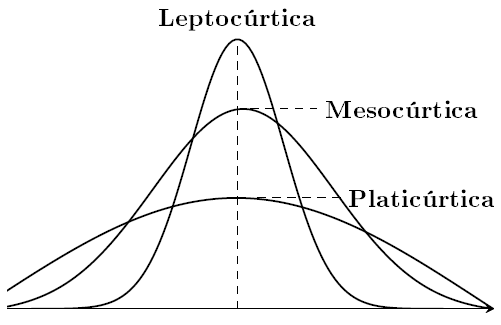
\includegraphics[scale=.9]{figuras/curtose}
\end{figure}
\subsubsection{Grau de curtose}
\inic Para medir o grau de curtose utiliza-se o coeficiente:
	\begin{equation}
	K = \frac{Q_1-Q_3}{2(P_{90} - P_{10})},    
	\end{equation}
	considerando a classificação:
	\begin{enumerate}
		\item[(i)] Se $K =0,263$, diz-se distribuição mesocúrtica; 
		\item[(ii)] Se $K>0,263$, diz-se distribuição platicúrtica;
		\item[(iii)] Se $K<0,263$, diz-se distribuição leptocúrtica.
	\end{enumerate}
\noindent \exemplo

\begin{enumerate}
	\item[(i)] Num teste aplicado a 20 alunos, obteve-se a seguinte distribuição de pontos:
	\begin{equation*}
	    \begin{tabular}{|c|c|c|c|c|c|c|c}
		    35 $\vdash$ 45 & 45 $\vdash$ 55 & 55 $\vdash$ 65 & 65 $\vdash$ 75 & 75 $\vdash$ 85 & $85 \vdash \hspace{-0.2 cm }\dashv 95$ \\ 
		    \hline
		    1&3&8&3&3&2\\
	    \end{tabular}
	\end{equation*}
	\begin{enumerate}
		\item[(a)] Calcular o desvio médio; 
		\item[(b)] Determinar a variância populacional;
		\item[(c)] Determinar o desvio padrão;
		\item[(d)] Classifique a distribuição quanto a assimetria e curtose.
	\end{enumerate}
\end{enumerate}
	
% \section{Teorema da Probabilidade Total}
% \section{O Teorema de Bayes}
% \section{Variáveis aleatórias}
% \subsection{Distribuição de probabilidade}
% \subsection{Esperança Matemática}
% \subsection{Variância}
% \chapter{Amostragem}

% \chapter{Teoria da Estimação}

% \chapter{Teoria da Decisão}

% \chapter{Modelos de Regressão}

% \chapter{Aplicações}

% \section{Aplicações à Administração}
% \section{Aplicações à Física}
% \section{Aplicações à Análise de Reflorestamento}
% \section{Aplicação à Propagação de Doenças}